\documentclass[tikz,border=5pt]{standalone}
\usepackage{amsmath,amssymb}
\begin{document}
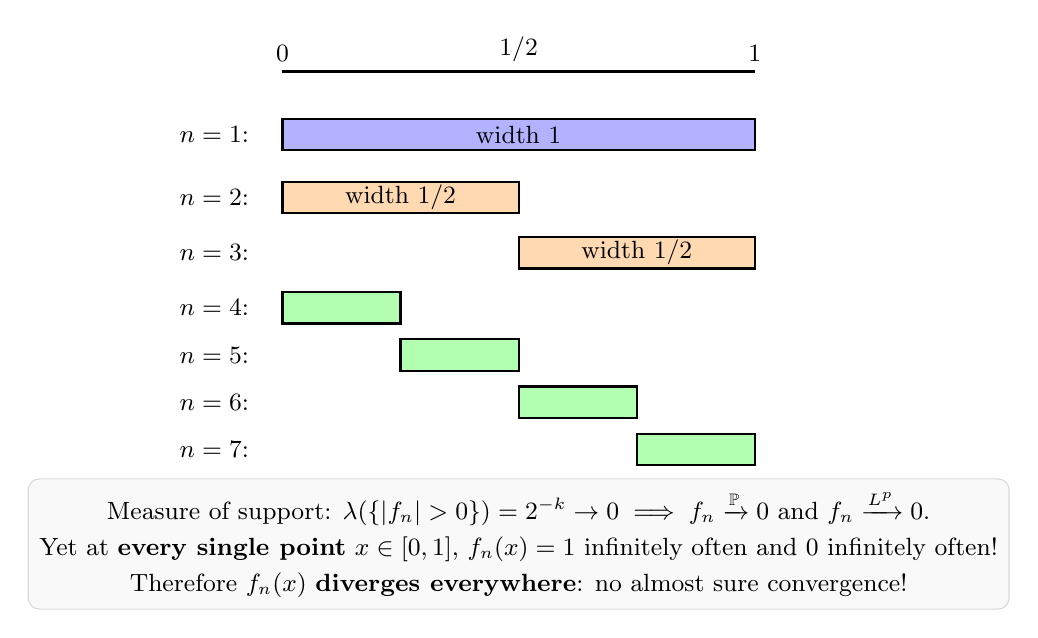
\begin{tikzpicture}[>=latex, font=\small]
  % Axis header
  \draw[thick] (0, 4.8) -- (6, 4.8);
  \node[above] at (0, 4.8) {$0$};
  \node[above] at (3, 4.8) {$1/2$};
  \node[above] at (6, 4.8) {$1$};

  % Level 0
  \node[left] at (-0.3, 4.0) {$n=1$:};
  \draw[thick, fill=blue!30] (0, 3.8) rectangle (6, 4.2);
  \node at (3, 4.0) {width $1$};

  % Level 1
  \node[left] at (-0.3, 3.2) {$n=2$:};
  \draw[thick, fill=orange!30] (0, 3.0) rectangle (3, 3.4);
  \node at (1.5, 3.2) {width $1/2$};

  \node[left] at (-0.3, 2.5) {$n=3$:};
  \draw[thick, fill=orange!30] (3, 2.3) rectangle (6, 2.7);
  \node at (4.5, 2.5) {width $1/2$};

  % Level 2
  \node[left] at (-0.3, 1.8) {$n=4$:};
  \draw[thick, fill=green!30] (0, 1.6) rectangle (1.5, 2.0);

  \node[left] at (-0.3, 1.2) {$n=5$:};
  \draw[thick, fill=green!30] (1.5, 1.0) rectangle (3, 1.4);

  \node[left] at (-0.3, 0.6) {$n=6$:};
  \draw[thick, fill=green!30] (3, 0.4) rectangle (4.5, 0.8);

  \node[left] at (-0.3, 0.0) {$n=7$:};
  \draw[thick, fill=green!30] (4.5, -0.2) rectangle (6, 0.2);

  \node[align=center, fill=gray!5, draw=gray!30, rounded corners, inner sep=4pt] at (3.0, -1.2)
    {Measure of support: $\lambda(\{|f_n| > 0\}) = 2^{-k} \to 0 \implies f_n \xrightarrow{\mathbb{P}} 0$ and $f_n \xrightarrow{L^p} 0$.\\[2pt]
     Yet at \textbf{every single point} $x \in [0,1]$, $f_n(x) = 1$ infinitely often and $0$ infinitely often!\\[2pt]
     Therefore $f_n(x)$ \textbf{diverges everywhere}: no almost sure convergence!};
\end{tikzpicture}
\end{document}
